% Magic comment to tell latex to compile with lualatex
% !TeX program = lualatex

\documentclass[11pt,a4paper]{article}

\usepackage{indentfirst}
\usepackage{shellesc,xpatch}
\usepackage[french]{translator}
\usepackage{float}
\usepackage{glossaries} % Pour faire des glossaires
\usepackage{natbib} % Pour créer des références bibliographiques
\usepackage{comment} % Pour les commentaires
\usepackage{graphicx} % Pour les images
\usepackage[french]{babel} % Document FR
\usepackage[T1]{fontenc} % Document FR
\usepackage{fontspec} 
\usepackage{fancyhdr} % Pour des en-tête et pied de page stylé
\usepackage{url} % Pour afficher les URL
\usepackage{appendix} % Pour les annexes
\usepackage{listings} % Pour les tables de code.
\usepackage{eso-pic}
\usepackage{wrapfig}
\usepackage{todonotes} % Pour les TODO
\usepackage{xcolor} 
\usepackage[cache=false]{minted} % Pour afficher du code proprement. Besoin de rajouter cache=false pour corriger un bug dans minted
\usepackage[normalem]{ulem} 
\usepackage{enumerate} % Des listes numérotées.
\usepackage{pdfpages}
\usepackage{epigraph}

\usepackage{lipsum} % only for demonstrating purpose, you can safely remove this package
%% \lipsum
%% \lipsum[3-56] 

\usepackage{tikz}
\usetikzlibrary{calendar}
\usepackage{placeins}
\usepackage{textcomp}
\usepackage{pgfgantt}


% Définitions des titres
\renewcommand\listoflistingscaption{Liste des codes sources}
\renewcommand\listingscaption{Code}

% pour switch auto papier / pdf
\newtoggle{paper}

% Pick one and comment the other one.
% \toggletrue{paper}
\togglefalse{paper}

\iftoggle{paper}{%
	% paper
	\usepackage[left=6cm,right=4cm,top=4cm,bottom=4cm]{geometry} % Pour le rapport imprimé 
}{%
	% electronic
	\usepackage[left=3cm,right=3cm,top=3cm,bottom=3cm]{geometry}
}

% Gestion des marges. Lien utile.
% https://www.debian-fr.org/t/latex-definir-un-paragraphe-en-dehors-des-marges/13991/3

% Réglages d'affichage
\setcounter{tocdepth}{3} % granularité de la table des matières
\setlength{\parindent}{3em} % On modifie l'indentation des paragraphes
\setlength{\parskip}{1em} % On modifie l'espace entre les paragraphes
\widowpenalty=10000 % Pour les veuves et les orphelines
\clubpenalty=10000 % Pour les veuves et les orphelines
\FrenchFootnotes %% FROM : http://www.xm1math.net/doculatex/notesbasdepage.html
\newcommand{\numerotationType}{arabic} %Type de numérotation : Roman ou arabic

%% FROM http://forum.mathematex.net/latex-f6/glossaire-t8654.html#p85429
\renewcommand{\glstextformat}[1]{#1*} % Affichage dans le corps du texte d'une entrée du glossaire


%%%%%%%%%%%%%%%%%%%%%%%%%%%%%%%%%%%%%%%%%%%%%%%%%%%%%%%%%%%%%%%%%%%%%%%%%%%%%%%%%%%%%%%%%%%%%%
\begin{comment}
	Fonction utilisée pour insérer une image. L'image doit être située dans le répertoire "img"
	Paramètres : 
	#1 : Positionnement de l'image [Paramètre optionnel]
			H 	Place le flottant ici, c'est-à-dire à l'endroit auquel il apparaît dans le texte source.
			t 	Position en haut de la page.
			b 	Position en bas de la page.
			p 	Place sur une page particulière réservée aux flottants.
			! 	Passe outre les paramètres internes que Latex utilise pour déterminer une position optimale des flottants. (déconseillé)
	#2 : échelle de l'image
	#3 : nom absolu du fichier (extension du fichier comprise)
	#4 : Commentaire affiché sous l'image
	#5 : id de l'image (utile pour y faire référence par la suite)
	Exemple d'utilisation :
	\newImage{2}{test.png}{ceci est un test}{test} : Laisser LateX se demerder pour placer au mieux
	\newImage[H]{2}{test.png}{ceci est un test}{test} : Forcer le placement de l'image à cet endroit exact.
\end{comment}
\newcommand{\newImage}[5][h]
{
\begin{figure}[#1]
    \centering
    \includegraphics[scale=#2]{img/#3}
    \caption{#4}
    \label{fig:#5}
\end{figure}
}

%%%%%%%%%%%%%%%%%%%%%%%%%%%%%%%%%%%%%%%%%%%%%%%%%%%%%%%%%%%%%%%%%%%%%%%%%%%%%%%
% Same as before, but annexe without captions.
\newcommand{\newImageAnnexe}[4][h]
{
\begin{figure}[#1]
    \centering
    \includegraphics[scale=#2]{img/#3}
    \label{annexe:#4}
\end{figure}
}

%%%%%%%%%%%%%%%%%%%%%%%%%%%%%%%%%%%%%%%%%%%%%%%%%%%%%%%%%%%%%%%%%%%%%%%%%%%%
\begin{comment}
	Fonction utilisée pour ajouter une URL.
	@see http://timmurphy.org/2010/04/04/referencing-website-urls-with-latex-bibtex/ ?
	Paramètres : 
	#1 : url (doit OBLIGATOIREMENT faire référence à un id de main.bib)
	#2 : Nom donné
	Exemple d'utilisation :
	\addURL{www.google.fr}{Google}
\end{comment}
\newcommand{\addURL}[2]
{
#2\footnote{#1 (cf. entrée \cite{#1} des références)}
}

%%%%%%%%%%%%%%%%%%%%%%%%%%%%%%%%%%%%%%%%%%%%%%%%%%%%%%%%%%%%%%%%%%%%%%%%%%%%%
\begin{comment}
	Fonction pour ajouter un acronyme contenant une définition au glossaire.
	Paramètres : 
	#1 : id acronyme
	#2 : Nom acronyme court
	#3 : Nom complet acronyme
	#4 : Description dans le glossaire

	Exemple d'utilisation :
	\newAcronym{API}{API}{Application Programming Interface}{Définition de API}
\end{comment}
\newcommand{\newAcronym}[4]
{
	\newglossaryentry{#1}
	{
			name={#2},
			description={#4},
			first={\glsentrylong{#1} (#2)},
			long={#3}
	}
}

%%%%%%%%%%%%%%%%%%%%%%%%%%%%%%%%%%%%%%%%%%%%%%%%%%%%%%%%%%%%%%%%%%%%%%%%%%%%%%%%%%%%%%%%%%%%%%
% http://www.developpez.net/forums/d961640/autres-langages/autres-langages/latex/mise-forme/referencer-annexe/#post5400726
% Pas un grand intérêt, mais à garder sous le coude, on sait jamais.
\newcommand{\annexe}[1]{annexe~\ref{#1} (page~\pageref{#1})}
%%%%%%%%%%%%%%%%%%%%%%%%%%%%%%%%%%%%%%%%%%%%%%%%%%%%%%%%%%%%%%%%%%%%%%%%%%%%%%%%%%%%%%%%%%%%%%
\begin{comment}
	Quelques commandes utiles pour la compilation avec un index ou des références.
	
	Build Glossaries
		- "makeindex.exe -s main.ist -t main.glg -o main.gls main.glo"
	
	Build References
	- "bibtex main"
	
	Exemple bibliographie dans le fichier main.bib :
	\@Misc{ 
		google, % Identifiant pour y faire références
		note = {}, % Une note optionnelle
		title = {Google}, % Titre
		author = {\url{google.com}} % Lien vers URL ou titre du livre.
	}
	
	Créer des tableaux LateX facilement
	http://www.tablesgenerator.com
	
\end{comment}

%%%%%%%%%%%%%%%%%%%%%%%%%%%%%%%%%%%%%%%%%%%%%%%%%%%%%%%%%%%%%%%%%%%%%%%%%%%%%%%%%%%%%%%%%
% This is where the magic happens..
\newcommand{\nocontentsline}[3]{}
\newcommand{\tocless}[2]{\bgroup\let\addcontentsline=\nocontentsline#1{#2}\egroup}

% Définir le titre des annexes dans le sommaire (ne marche pas si mis dans parameters)
\renewcommand{\addappheadtotoc}{Annexes}

% Création glossaire
\makeglossaries
% Chargements des entrées du glossaire. APRES \makeglossaries
\loadglsentries{glossaire.tex}

% Début du document
\begin{document}	
	\pagestyle{plain} % Juste le numero de page pour en-tête / pied de page.
	\pagenumbering{gobble} % pas de numérotation
	%%%%%%%%%%%%%%%%%%%%%%%%%%%%%%%%%%%%%%%%%
% University Assignment Title Page 
% LaTeX Template
% Version 1.0 (27/12/12)
%
% This template has been downloaded from:
% http://www.LaTeXTemplates.com
%
% Original author:
% WikiBooks (http://en.wikibooks.org/wiki/LaTeX/Title_Creation)
%
% License:
%% CC BY-NC-SA 3.0 (http://creativecommons.org/licenses/by-nc-sa/3.0/)
% 
% Instructions for using this template:
% This title page is capable of being compiled as is. This is not useful for 
% including it in another document. To do this, you have two options: 
%
% 1) Copy/paste everything between \begin{document} and \end{document} 
% starting at \begin{titlepage} and paste this into another LaTeX file where you 
% want your title page.
%% OR
% 2) Remove everything outside the \begin{titlepage} and \end{titlepage} and 
% move this file to the same directory as the LaTeX file you wish to add it to. 
% Then add \input{./title_page_1.tex} to your LaTeX file where you want your
% title page.
%
%%%%%%%%%%%%%%%%%%%%%%%%%%%%%%%%%%%%%%%%%

\begin{titlepage}

\newcommand{\HRule}{\rule{\linewidth}{0.5mm}} % Defines a new command for the horizontal lines, change thickness here

\center % Center everything on the page
 
%----------------------------------------------------------------------------------------
%%	HEADING SECTIONS
%----------------------------------------------------------------------------------------
\begin{minipage}{0.4\textwidth}
	\begin{flushleft} \large
		EPSI Bordeaux\\
		114 Rue Lucien Faure\\
		33000 Bordeaux
	\end{flushleft}
\end{minipage}
~
\begin{minipage}{0.4\textwidth}
	\begin{flushright} \large
		\onepoint\\
		28 Avenue Léonard de Vinci \\
		33600 PESSAC
	\end{flushright}
\end{minipage}\\[2cm]


\textsc{\LARGE EPSI Bordeaux - 5\up{ème} année}\\[1.0cm]

\space

\HRule \\[0.4cm]
{ \huge \bfseries 
Comment l'automatisation peut permettre de réduire les erreurs humaines dans la mise en oeuvre d'une application ?
}\\[0.4cm]
\HRule \\[1.5cm]

\LARGE Sylvain \textsc{METAYER}\\[2cm] % Your name

\begin{flushleft} \large
	\emph{Tuteur Entreprise :}\\
	Nicolas \textsc{GUERINET}
	\newline\newline
	\emph{Tuteur EPSI :} \\
	Sylvain \textsc{LABASSE}
\end{flushleft}


\includegraphics[scale=0.2]{img/epsi.png}\\[1cm] % Include a department/university logo - this will require the graphicx package


\includegraphics[scale=0.05]{img/onepoint.png}\\[1cm] % Include a department/university logo - this will require the graphicx package

\begin{flushright} \large 
	Promotion 2019, Soutenu en Septembre 2019
\end{flushright}

\vfill % Fill the rest of the page with whitespace

\end{titlepage} 
\newpage
	~ % Hide summary page.
\newpage
	%% TODO Listing. Comment this page before printing !
	\listoftodos 
\newpage
	% Define Sommaire instead of "Table of Content"
	\renewcommand{\contentsname}{Sommaire}
	\tableofcontents
\newpage
	\pagenumbering{\numerotationType} % start numerotation
	\section*{Introduction}
	\addcontentsline{toc}{section}{Introduction} % ajout de la référence dans la table des matières
	\todo{Introduction, 5-6 pages}

\todo{Quand la partie introduction sera terminée, supprimer les parties.}

\subsection{Accroche}
L'automatisation a toujours été perçue comme un moyen de gagner en productivité, temps, et donc de rendre des projets toujours plus rentable.
	
Les projets informatiques sont de plus en plus nombreux, que cela soit des logiciels de bureau, des applications web, ou encore avec les nouveaux terminaux, des applications mobile, tablettes ou même pour montres connectées.
	
Les projets augmentent donc en quantité, mais augmentent-ils en qualité ? Leur fiabilité n'est en effet pas toujours optimale. 
	
Combien de projet sont encore déployé manuellement car aucune automatisation n'est présente sur le projet ? 
	
En plus d'une perte de temps, parfois importante, cela engendre un stress au niveau des équipes de développeurs, qui à chaque livraison redoute les régressions qui pourraient survenir ou encore les bugs de déploiement.

L'automatisation peut également permettre d'améliorer l'arrivée d'un nouveau développeur sur un projet. Il n'est en effet par rare de voir des projets ou la configuration de l'environnement requiert à elle seule plusieurs jours, sans que le développeur puisse vraiment commencer à travailler.
	
L'automatisation va permettre d'améliorer la fiabilité ainsi que la confiance des développeurs et clients dans le projet, puisque des tests automatisés ainsi qu'une chaine d'industrialisation complètement automatisée permet ainsi de déployer avec confiance une application.
	
Nous allons donc tenter de répondre à la problématique suivante :
	
{\LARGE \problematique}

\subsection{Définition}

Avant de continuer, il convient de s'attarder sur ce qu'est l'automatisation.

Selon le Larousse, l'automatisation est le 

\begin{quote}
fait d'automatiser l'exécution d'une tâche, d'une suite d'opérations...
\end{quote}

\subsection{Historique}

Idées : 
	
- Mode opératoire suivi religieusement, 

- script expect

- Comment déployait-on avant ?

-  ...


\textit{L’introduction doit remplir une fonction traditionnelle : délimiter et présenter le projet ou la mission et son contexte professionnel, annoncer les parties principales du développement. L’introduction représente environ un dixième du mémoire. Il faut absolument insister sur la bonne impression qu’elle doit donner au lecteur comme premier et décisif contact avec le mémoire.}

\subsection{Que peut-on automatiser ?}

\subsection{Pourquoi automatiser ?}

Quels en sont les avantages ?

- éviter erreurs développeur

- éviter script executé avec mauvais parmaètres

\subsection{Présentation entreprise / mission}

L'entreprise dans laquelle j'effectue mon alternance depuis septembre 2017 est \onepoint. 

\xmakefirstuc{\onepoint{}} est une \gls{esn} à taille humaine. Son domaine d'activité est d'accompagner ses clients dans leur transformation numérique, 

C'est une \gls{SAS} disposant de 14 implantations dans le monde. L'entreprise a effectué en 2018 un chiffre d'affaire de 300 million d'euros.

Elle dispose de 2300 collaborateurs, en moyenne agé de 33 ans.

\xmakefirstuc{\onepoint{}} se compose de plusieurs communautés.

\begin{itemize}
	\item Des communautés \emph{régions}, permettant de regrouper les collaborateurs par leur proximité géographique.
	\item Des communautés \emph{expertise}, regroupant l'expertise de chacun, et permettant à tous de progresser. On y retrouve par exemple la communauté Sécurité ou encore Architecture.
	\item Des communautés \emph{support}, tel que la \gls{DSI}, ou les Ressources Humaines, nécessaire au fonctionnement de l'entreprise.
	\item Des communautés \emph{métiers}, regroupant des personnes maitrisant les aspects métiers des différents clients, ainsi que les contraintes de ces métiers. Cela peut par exemple être les métiers des Assurances, des Banques, des Télécoms... 
\end{itemize}

Ainsi, lors du développement d'un projet, toutes ces communautés sont utilisés, afin de tirer le meilleur d'entre elle et de regrouper les personnes les plus aptes à réaliser le projet.

Cela implique aussi que chaque collaborateur peut ainsi appartenir à une ou plusieurs communautés, selon ses compétences, expérience et localisation.

\subsubsection{Historique} 

\xmakefirstuc{\onepoint{}} a été créé en 2002, par David Layani.

De 2003 jusqu'en 2007, elle va s'ouvrir à l'international, avec l'ouverture de bureaux au Canada, en Chine et en Tunisie.

En 2008, elle étend sa position en France, avec l'ouverture de deux centres de production, à Bordeaux et Nantes.

En 2015, \onepoint{} continue son développement international au Luxembourg, en Belgique et en Hollande, avant de racheter VisionIT Group.

En 2018, \onepoint{} ouvre des bureaux à Lyon et en Australie, et rachète également Weave ainsi que Géronimo, acteur important dans la conception d'application mobile.

\subsubsection{Réalisations}

\subsubsection{Contexte de l'alternance}

Projet Nouvelle Aquitaine, chaine d'industrialisation pour pouvoir permettre déploiement de multiple sites Drupal.

\textit{Projet \bv{}, ou il y a une architecture actuelle qui n'est pas satisfaisante pour X raisons (reproductibilité...), et qui doit être changé}.

\textit{Elaborer un schéma directeur à partir d’orientations stratégiques} => Conduite de changement


\subsection{Annonce du plan}
\newpage
	%%%%%%%%%%%%%%%% FANCY %%%%%%%%%%%%%%%%%
	% Fancy header / footer
	\pagestyle{fancy}
	
	% Obtenir le nom de la section/sous-section sans le numero
	\renewcommand{\sectionmark}[1]{\markright{#1}}
	\renewcommand{\subsectionmark}[1]{\markright{#1}}
	\renewcommand{\subsubsectionmark}[1]{\markright{#1}}
	
	%% HEADER
	%\renewcommand{\headrulewidth}{0.4pt}
	\lhead{\fancyplain{}{}}
	\chead{\fancyplain{}}
	\rhead{\fancyplain{}{\rightmark}}
	
	%% FOOTER
	%\renewcommand{\footrulewidth}{0.4pt}
	\lfoot{\fancyplain{}{}}	
	\cfoot{\fancyplain{}{}}	
	\rfoot{\fancyplain{}{\thepage}}
	%%%%%%%%%%%%%%%% END FANCY %%%%%%%%%%%%

  \section{Contexte}
	\subsection{Subsection example}
	\subsubsection{Subsubsection example}

\begin{itemize}
	\item A
	\item B
\end{itemize}

\clearpage
\newpage
	\section{Main Content}
	\subsection{Project presentation}
	Table example : 

% Créer des tableaux LateX facilement
% http://www.tablesgenerator.com
\begin{table}[H] % Le paramètre H (majuscule) signifie : place cet élément à cet endroit précisement.
\centering
\begin{tabular}{|c|l|l|l|}
\hline
\textbf{Utilisateur} & \multicolumn{1}{c|}{\textbf{Version 1}} & \multicolumn{1}{c|}{\textbf{Version 2}} & \multicolumn{1}{c|}{\textbf{Version 3}} \\ \hline
\textit{Pierre} & Non & Non & Oui \\ \hline
\textit{Paul} & Oui & Oui & Non \\ \hline
\textit{Jacques} & Oui & Oui & Non \\ \hline
\textit{Hector} & Oui & Oui & Oui \\ \hline
\end{tabular}
\caption{Accès des différents utilisateurs aux différents versions}
\label{tab:versions}
\end{table}
\subsubsection{Task 1}
	\newImage[H]{0.05}{image.jpg}{Image example}{image-example}

\begin{itemize}
	\item A
	\item B
	\item C
\end{itemize}


\begin{enumerate}
	\item A
	\item B
\end{enumerate}

\paragraph*{Reference to annexes, bibliography URL \& Glossary items}

	Hello (cf. annexe \ref{code:php-example})
	
	Here is a link example \addURL{http://google.com}{My custom Text}.
	
	Acronym example : \gls{HTML}


\subsubsection{Task 2}
	
\begin{listing}[H]
	\caption{Example of PHP Code}
	\inputminted[breaklines,linenos]{php}{code/entity.php}
	\label{code:entity}
\end{listing}


\begin{listing}[H]
	\caption{Exemple Markdown}
	\inputminted[breaklines,linenos]{php}{code/markdown.md}
	\label{code:markdown}
\end{listing}
\clearpage
\newpage
	\pagestyle{plain} % Juste le numero de page pour en-tête / pied de page à partir de maintenant
	\section*{Conclusion}
	\addcontentsline{toc}{section}{Conclusion} % ajout de la référence dans la table des matières
	\todo[color=yellow]{Conclusion, 7 pages}

- Pourquoi n'existe pas une solution unique ? => car chaque projet différent 

- Pourquoi complexité des processus de déploiement ? => car complexité application en hausse, et demande utilisateur avec toujours plus de simplicité, et donc complexe à réaliser. Passage d'une "application à la bonne franquette", à un vrai processus éprouvé pour durer

\subsection{Bénéfices}

\todo[color=orange]{Benefices}

\textit{dentifier les leviers d’économie à actionner pour améliorer les processus Qualité.}

\begin{itemize}
	\item KPI à trouver
	\item Confiance dans la livraison
	\item ROI avec rapidité de livraison
	\item Décharge l'équipe
	\subitem Plus de temps pour de la valeur métier
	\item L'automatisation peut permettre de relancer rapidement une activité défaillante (SLA / PRA / PCA)
\end{itemize}

\begin{itemize}
	\item - Erreur développeur
	\item + de Fiabilité
	\item Preuve de qualité
	\item Time To Market réduit
	\item Reproductibilité
\end{itemize}

Comment faire en sorte que ça marche dans la durée ? Des controles / supervisons périodique afin de checker que tout va bien.

Workflow : savoir ce qui est automatisé, comment c'est mis en oeuvre ,documentation des outils, ...
Faire en sorte que l'automatisation ne casse pas et que l'on en tire quelques chose, que l'on soit nouvel arrivant sur le projet, ou développeur déjà présent sur le projet.

Scalabilité : Docker / provisionner de nouveaux serveurs rapidement avec Ansible par exemple.

Déploiement : chaine de déploiement (dev/test/inte/preprod/prod) avec chacune ses spécificités

Exemple :

en dev, on souhaite des logs direct dans la console, en prod on les mets dans un fichier de log.
en dev, on veut le mode debug, en prod on le désactive.

\subsection{Limites}

\todo[color=yellow]{Limites}

Sur-qualité, sur-optimisation, ...

Aucun intérêt si les tests ne sont pas fiable.

Dépend du client, de l'environnement, demande de la flexibilité, délai de mise en place, ROI

Pré-requis à l'automatisation

Attention, auto != vérité \url{https://www.matuzo.at/blog/building-the-most-inaccessible-site-possible-with-a-perfect-lighthouse-score/}

L'automatisation ne peut être utilisée, ou sera risquée, ou plus à même d'amener des régression si de mauvaise pratique sont présentes.

\begin{itemize}
	\item variable codée en dur à la place de variable d'environnement
	\item ...
\end{itemize}

De plus, il faut une certaine organisation.

Cela peut-être perçu comme une perte de temps par certaines personnes (hiérarchie, manager, ...), qui y verrons la une perte d'argent et de temps par exemple. Il faut alors pouvoir montrer que cela est rentable, au travers de \gls{KPI} bien déterminé.

Le fait d'automatiser des processus permet de gagner du temps, et par conséquent de l'argent et de consacrer ses efforts à d'autres taches qui peuvent apporter de la valeur métier.

Le coût horaire libéré, calculer à partir de combien de temps il est rentable.

Par exemple, une tache à 3000€ qu'on automatise et qui ne coute plus que 300€ est rentable en 10 semaines.

Facteur humain : Le temps libéré par l'automatisation des tâches peut permettre de souder les liens d'une équipe et d'améliorer les relations de cette dernière. Cela libère du temps pour du team building par exemple.

Un sujet technique qui rapproche en terme d'humain

Idées de \gls{KPI} en vracs.

Métrique - KPI - temps de déploiement / nombre d'incident / uptime / Nombre de build KO / Nombre de build OK ... permettent de définir l'impact des services mis en place sur le S.I

\begin{itemize}
	\item temps de déploiement
	\item taux de déploiement succès
	\item couverture de code
	\item tests au verts
	\item derniers build KO
\end{itemize}

Parler de l'importance de l'implication du client. 

Ex :  Rédaction de SFD, qui évolue tout les 4 matins, et demande un changement dans l'architecture => automatisation perdante.

Dépôt git du mec qui automatise tout \url{https://github.com/NARKOZ/hacker-scripts}

\subsection{Ce qui n'est pas encore automatisé}

\subsection{Les possiblités d'automatisation dans le futur}

\textit{Parler de ce qui n'est pas encore automatisé, et les différentes pistes d'automatisation possible dans le futur.}



\newpage
	\addcontentsline{toc}{section}{Glossaire, références, tables des codes, des figures, des tableaux et annexes}
	\glsaddall % ajouter toutes les entrées n'ayant pas encore été citées
  \printglossaries % afficher le glossaire
\newpage
	\nocite{*} % Add all bibliography items that have not been listed yet.
	\bibliographystyle{unsrt} 
	\bibliography{main}{}
	\clearpage

	\listoffigures 
	\listoflistings
	\listoftables
\newpage
	\pagenumbering{gobble} % No numerotation
	\vspace*{\stretch{1}}
		\begin{center}
			\begin{Huge}
				\section*{\MakeUppercase{Annexes}} 
			\end{Huge}
		\end{center}
	\vspace*{\stretch{1}}
\newpage
	\appendix % Annexes with A, B, C, D numerotation
	\section{Schéma simplifié du cycle de vie d'un projet}
\newImageAnnexe[H]{0.75}{cycle-vie-projet.png}{cycleVieProjet}

\clearpage
\section{Construction des modules communs de l'application au sein d'un projet \naq}
\newImageAnnexe{0.9}{modules.png}{commons-modules}

\clearpage
\section{Build continu d'un projet \naq}
\begin{figure}[ht]
	\centering
	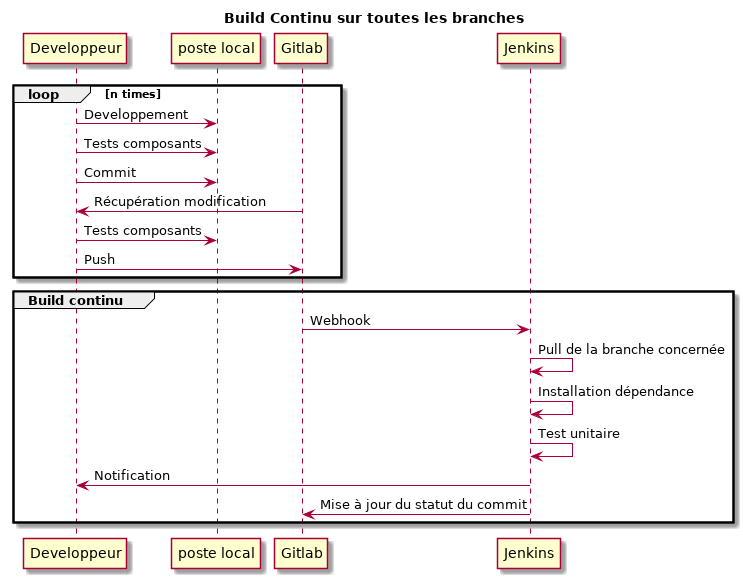
\includegraphics[scale=0.6,angle=-90]{img/build-continu.png}
	\label{annexe:build-continu}
\end{figure}

\clearpage
\section{Flux de travail du déploiement d'une version d'un site \naq}
\newImageAnnexe{0.32}{release.png}{release-naq}

\clearpage
\section{Matrice de développement \devops}

\normalsize{Source : \url{https://www.infoq.com}}

\begin{figure}[ht]
	\centering
	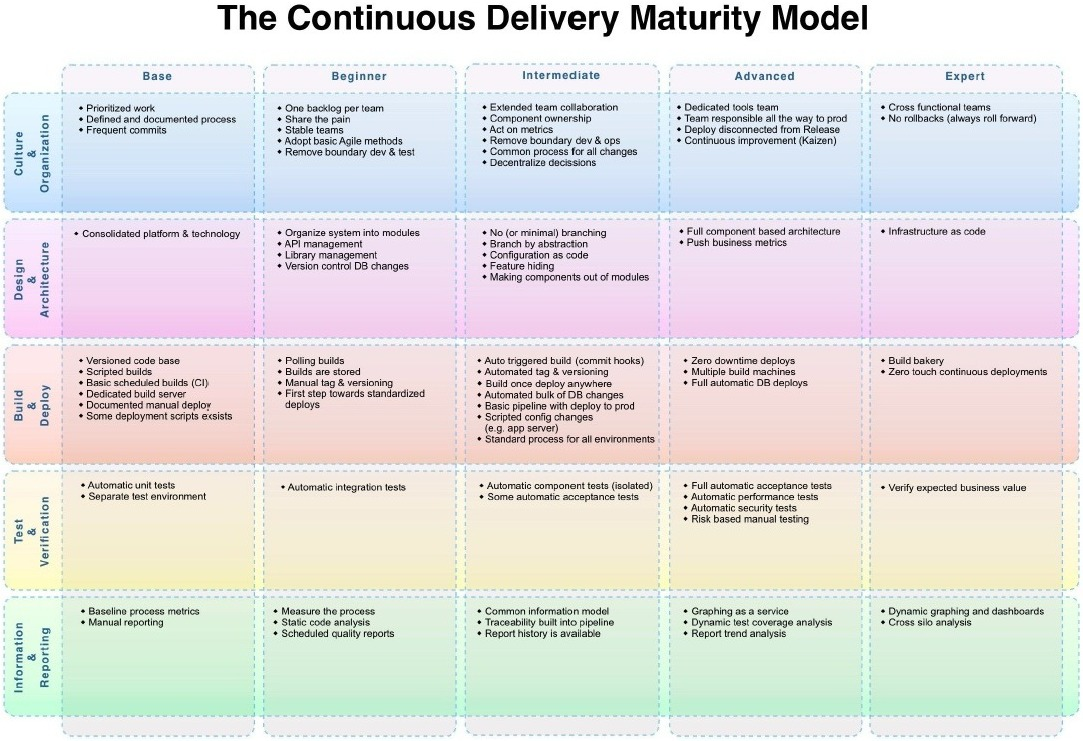
\includegraphics[scale=0.62,angle=-90]{img/devops-matrice.jpg}
	\label{annexe:devops-matrice}
\end{figure}

\clearpage
\section{Exemple d'erreurs détectées par PHPStan}

Dans l'exemple ci-dessous, PHPStan retournera une erreur indiquant que le paramètre requis \frquote{\$type} n'a pas été renseigné, ainsi qu'une erreur indiquant que la méthode privée \frquote{internalBehaviour} ne peut être utilisée en dehors de la classe. 

Il est à noter que cette analyse statique de code peut être et est souvent effectuée au sein de l'\gls{IDE} pour permettre une détection de l'erreur au plus tôt.

\begin{minted}[linenos]{php}
<?php
// index.php

require_once(__DIR__."/vendor/autoload.php");
$a = new \App\File();
$content = $a->loadFile("file.json");
$a->internalBehaviour();

// src/File.php

namespace App;

class File {
  public function loadFile($file, $type) {
    $content = file_get_contents($file);
    if ($type == "json") {
      return json_decode($file);
    }
    return $content;
  }
  
  private function internalBehaviour() {
    echo "this is not public";
  }
}

// ------ ------------------------------------------------------------------- 
// Line   index.php                                                          
// ------ ------------------------------------------------------------------- 
// 6      Method App\File::loadFile() invoked with 1 parameter, 2 required.  
// 7      Call to private method internalBehaviour() of class App\File.      
// ------ ------------------------------------------------------------------- 

\end{minted}
\label{annexe:php-error}


%\clearpage
%\section{Flux de travail pour un hotfix sur un site \naq}
%\newImageAnnexe{0.25}{hotfix.png}{hotfix-naq}
\end{document}